\documentclass{beamer}
\usepackage[francais]{babel}
\usepackage[T1]{fontenc}
\usepackage[utf8]{inputenc}
\usepackage{graphicx}
\usepackage{multirow}
\usetheme[secheader]{Madrid}    % titre en haut
\useoutertheme{infolines}       %ligne d'en-tête et de pied de page
\definecolor{vert}{HTML}{088A08} % vert 
\definecolor{brun}{HTML}{BD8D46} % brun 
\setbeamercolor{structure}{fg=vert}

\title{GTK+ une alternative à Qt}
\author{Daniel Antunes}
\date{\today}

\begin{document}

\begin{frame}
  \begin{center}
  
\includegraphics[scale=0.39]{logo.png}
  \end{center}
  \titlepage
\end{frame}

\begin{frame}
  \frametitle{Table des matières}
  {\small \tableofcontents[hideallsubsections]}
\end{frame}

\section{Introduction}

\begin{frame}
  \frametitle{Introduction à GTK+}
  
  \begin{itemize}
  \item GTK+: \textbf{G}IMP \textbf{T}ool\textbf{k}it
  \item librairie pour création d'interface graphique
  \item écrit en C
  \item compatible avec: C/C++, Java, Python, Perl, Ada, Fortan,...
  \item utilisable avec \textbf{Glade}
  \end{itemize}
  
\end{frame}

\section{GTK+ vs. Qt}

\begin{frame}
  \frametitle{GTK+ vs. Qt}
  \begin{tabular}{|c|c|}
  \hline
  GTK+ & Qt \\
  \hline \hline 
  combine bien avec GLib, GIO, & possède de nombreux modules: \\
  GStreamer, Pango et Cairo & QtSql, QtXml, QtWebkit, ... \\
  \hline
  \multirow{2}{*}{principaux systèmes d'exploitation} & principaux systèmes d'exploitation\\
   & + Android, iOS, Symbian, etc.\\
  \hline
  \multicolumn{2}{|c|}{performances identiques}\\
  \multicolumn{2}{|c|}{pour les mêmes tâches}\\
  \hline
  \multicolumn{2}{|c|}{utilisables sur $\sim$ mêmes langages}\\
  \hline
  $\sim$ 200 collaborateurs & $\sim$ 400 collaborateurs\\
  $\sim$ 3000 commits/an & $\sim$ 15000+ commits/an\\
  \hline
  \end{tabular}
\end{frame}

\section{Pour commencer...}

\begin{frame}
  \frametitle{Pour commencer...}
  \begin{itemize}
  \item Pour compiler Gtk+ en C, ajouter à la ligne de commande: \\
  \hspace{1cm}"\textcolor{blue}{\$(pkg-config --cflags --libs gtk+-2.0)}"
  \item Dans le programme: \\
  \hspace{1cm}"\textcolor{cyan}{\#}\textcolor{blue}{include} \textcolor{cyan}{<gtk/gtk.h>}"
  \item Ensuite, dans le main, il faut utiliser:\\
  \hspace{1cm}"\textbf{void} \textcolor{blue}{gtk\_init}(\textbf{int} *argc, \textbf{char} ***argv)"\\
  \textcolor{blue}{/*initialisation de GTK+ et éventuellement configuration si valeurs passées en paramètre du main*/}\\
  et plus tard:\\
  \hspace{1cm}"\textbf{void} \textcolor{blue}{gtk\_main}(\textbf{void})"\\
  \end{itemize}
\end{frame}

\subsection{Pour commencer... II}

\begin{frame}{Pour commencer... II (quelques notions)}
    \begin{itemize}
    \item Les widgets (\textbf{Wi}n\textbf{d}ow Gad\textbf{get}):\\
    \hspace{0.3cm}- objets GTK (notion d'héritage)\\
    \vspace{0.1cm}
    \hspace{0.3cm}- initialiser un objet: \\
    \hspace{0.5cm} GtkWidget *maFenetre;\\
    \hspace{0.5cm} maFenetre = \textcolor{blue}{gtk\_window\_new}(GTK\_WINDOW\_TOPLEVEL);\\
    \vspace{0.1cm}
    \hspace{0.3cm}- chaque type de widget a des fonctions de personnalisation de\\
    \hspace{0.4cm}  syntaxe: \textbf{type\_retour} \textcolor{blue}{gtk\_type\_effet} ( \textbf{paramètres} ); \\
    \hspace{0.4cm} où \textcolor{blue}{type} = type de widget (ex. window pour une fenêtre)\\
    \hspace{0.4cm} et \textcolor{blue}{effet} = action à éffectuer (ex. set\_relief, set\_title)\\
    \end{itemize}
\end{frame}

\subsection{Pour commencer... III}

\begin{frame}{Pour commencer... III (héritage GTK)}
GObject\\
+ - - GtkObject\\
|\hspace{0.8cm}+ - - GtkWidget\\
|\hspace{0.8cm}|\hspace{0.8cm}+ - - GtkContainer\\
|\hspace{0.8cm}|\hspace{0.8cm}|\hspace{0.8cm}+ - - GtkBin\\
|\hspace{0.8cm}|\hspace{0.8cm}|\hspace{0.8cm}|\hspace{0.8cm}+ - - GtkWindow\\
|\hspace{0.8cm}|\hspace{0.8cm}|\hspace{0.8cm}|\hspace{0.8cm}+ - - GtkButton\\
|\hspace{0.8cm}|\hspace{0.8cm}|\hspace{0.8cm}+ - - GtkToolbar\\
\vspace{0.3cm}
\textbf{\textcolor{blue}{\underline{Casting}}}\\
\vspace{0.2cm}
GTK\_WIDGET(widget)\hspace{1.1cm}GTK\_OBJECT(object)\\
GTK\_WINDOW(window)\hspace{0.8cm}GTK\_Container(container)\\
\end{frame}

\section{Des fenêtres et des boutons}

\begin{frame}{Des fenêtres et des boutons}
    \begin{itemize}
    \item création d'une fenêtre:\\
    \hspace{0.5cm}\textcolor{brun}{/* déclaration */}\\
    \hspace{0.5cm}GtkWidget *maFenetre;\\
    \hspace{0.5cm}\textcolor{brun}{/* initialisation */}\\
    \hspace{0.5cm}maFenetre = \textcolor{blue}{gtk\_window\_new}(GTK\_WINDOW\_TOPLEVEL);\\
    \hspace{0.5cm}\textcolor{brun}{/* affichage */}\\
    \hspace{0.5cm}\textcolor{blue}{gtk\_widget\_show}(maFenetre);\\
    \hspace{0.5cm}\textcolor{brun}{/* taille par défaut */}\\
    \hspace{0.5cm}\textcolor{blue}{gtk\_window\_set\_default\_size}(\textbf{GTK\_WINDOW}(maFenetre), 320 ,200);\\
    \vspace{0.2cm}
    \begin{itemize}
        \item GTK\_WINDOW\_TOPLEVEL: une fenêtre normale
        \item GTK\_WINDOW\_POPUP: une fenêtre vierge, sans bordures
    \end{itemize}
    les objets en GTK sont invisibles par défaut on peut utiliser:\\
    \hspace{0.5cm}\textbf{void} \textcolor{blue}{gtk\_widget\_show\_all} (\textbf{GtkWidget *}widget); 
    \end{itemize}
\end{frame}

\subsection{Des fenêtres et des boutons II}

\begin{frame}{Des fenêtres et des boutons II}
    \begin{itemize}
        \item création d'un bouton:\\
        \hspace{0.5cm}\textcolor{brun}{/* déclaration */}\\
        \hspace{0.5cm}GtkWidget *bouton;\\
        \hspace{0.5cm}\textcolor{brun}{/* initialisation */}\\
        \hspace{0.5cm}bouton = \textcolor{blue}{gtk\_button\_new}();\\
        \hspace{0.5cm}\textcolor{brun}{/* attacher le bouton à la fenêtre */}\\
        \hspace{0.5cm}\textcolor{blue}{gtk\_container\_add}(\textbf{GTK\_CONTAINER}(maFenetre),bouton);\\
        \vspace{0.3cm}
        pour l'initialisation de notre bouton on dispose de variantes:\\
        \begin{itemize}
            \item \textbf{GtkWidget*} \textcolor{blue}{gtk\_button\_new\_with\_label}(const \textbf{gchar *}label);
            \item \textbf{GtkWidget*} \textcolor{blue}{gtk\_button\_new\_with\_mnemonic}(const \textbf{gchar *}label);
            \item \textbf{GtkWidget*} \textcolor{blue}{gtk\_button\_new\_from\_stock}(const \textbf{gchar *}stock\_id);
        \end{itemize}
    \end{itemize}
\end{frame}

\subsection{D'autres widgets...}

\begin{frame}{D'autres widgets...}
    Exemples d'autres widgets:
    \begin{itemize}
        \item des GtkLabel, ils insèrent du texte dans l'interface graphique
        \item des GtkHBox/GtkVBox, permettent d'aligner des widgets horizontalement/verticalement
        \item des GtkTable, grille invisible pour la disposition des objets
        \item des GtkEntry, entrée de saisie
        \item des GtkImage, affichage d'images
        \item des boîtes de dialogue
        \item des GtkMenuBar/GtkMenuItem, barres de menu
        \item des GtkToolbar, barre d'outils (new, save, open,...)
        \item des GtkStatusBar, barre de status
        \item des GtkProgressBar, barre de progression
    \end{itemize}
\end{frame}

\section{Les signaux}

\begin{frame}{Les signaux}
    GTK+ fonctionne avec les principes des "signals" et fonctions "callback"\\
    \vspace{0.5cm}
    \begin{center}
    Action de l'utilisateur sur l'interface\\
    ||\\
    Réception d'un signal\\
    ||\\
    Réaction avec la fonction callback\\
    \end{center}
\end{frame}

\subsection{Les signaux II}

\begin{frame}{Les signaux II}
    Pour gérer tous ces évenements, une fonction:\\
    \vspace{0.1cm}
    \textbf{void} \textcolor{blue}{g\_signal\_connect} (\textbf{gpointer *}object, const \textbf{gchar *}name,\\
    \hspace{4cm}\textbf{GCallback} func, \textbf{gpointer} func\_data );\\
    \vspace{0.3 cm}
    \begin{itemize}
        \item object: le widget dont on veut gérer l'évenement, avec la macro G\_OBJECT(widget *) 
        \item name: une chaîne de caractères contenant le nom du signal, chaque signal possible a un nom
        \item func: une chaîne de caractères contenant le nom de la fonction callback qui sera appelée lors de l'émission du signal, avec la macro G\_CALLBACK
        \item func\_data: un pointeur vers d'éventuels paramètres de la fonction callback
    \end{itemize}
\end{frame}

\subsection{Les signaux III}

\begin{frame}{Les signaux III}
    Une fonction s'occupe de la boucle évènementielle:\\
    \begin{center}
        \textbf{void} \textcolor{blue}{gtk\_main} (\textbf{void});
    \end{center}
    Une seule façon d'y mettre fin:\\
    \begin{center}
        \textbf{void} \textcolor{blue}{gtk\_main\_quit} (\textbf{void});
    \end{center}
\end{frame}

\subsection{Exemple}

\begin{frame}{Exemple}
    \textcolor{blue}{g\_signal\_connect}(\textbf{G\_OBJECT}(boutonQuitter), \textcolor{magenta}{"clicked"},\\
    \hspace{3cm}\textbf{G\_CALLBACK}(maFonctionCallback), \textcolor{magenta}{NULL});\\
    \vspace{0.2cm}
    avec la fonction callback:\\
    \vspace{0.1cm}
    \textbf{void} \textcolor{blue}{maFonctionCallback}(\textbf{GtkWidget *}widget,\textbf{gpointer} data)\\
    \{\\
    \hspace{0.7cm}\textcolor{blue}{gtk\_main\_quit}();\\
    \}\\
\end{frame}

\section{GDK}

\begin{frame}{GDK}
    GDK:
    \begin{itemize}
    \item sous-bibliothèque de GTK+
    \item constituée principalement de fonctions de dessin
    \item permet de créer des interfaces pour des jeux
    \includegraphics[scale=0.35]{othello.png}
    \end{itemize}
\end{frame}

\subsection{GDK II}

\begin{frame}{Quelques fonctions GDK}
    \textcolor{brun}{/* dessiner un point */}\\
    \textbf{void} \textcolor{blue}{gdk\_draw\_point} (\textbf{GdkDrawable *}drawable, \textbf{GdkGC *}gc, \textbf{gint} x,\\
    \hspace{4cm}\textbf{gint} y);\\
    \textcolor{brun}{/* dessiner une ligne */}\\
    \textbf{void} \textcolor{blue}{gdk\_draw\_line} (\textbf{GdkDrawable *}drawable, \textbf{GdkGC *}gc, \textbf{gint} x1,\\
    \hspace{3.8cm}\textbf{gint} y1, \textbf{gint} x2, \textbf{gint} y2);\\
    \textcolor{brun}{/* dessiner un rectangle */}\\
    \textbf{void} \textcolor{blue}{gdk\_draw\_rectangle} (\textbf{GdkDrawable *}drawable, \textbf{GdkGC *}gc,\\
    \hspace{4.5cm}\textbf{gboolean} filled, \textbf{gint} x, \textbf{gint} y, \textbf{gint} width,\\
    \hspace{4.5cm}\textbf{gint} height);\\
    \textcolor{brun}{/* dessiner un arc ou un cercle (arc de 360 degrés) */}\\
    \textbf{void} \textcolor{blue}{gdk\_draw\_arc} (\textbf{GdkDrawable *}drawable, \textbf{GdkGC *}gc,\\
    \hspace{3.6cm}\textbf{gboolean} filled, \textbf{gint} x, \textbf{gint} y, \textbf{gint} width,\\
    \hspace{3.6cm}\textbf{gint} height, \textbf{gint} angle1, \textbf{gint} angle2);
\end{frame}

\subsection{GDK III}

\begin{frame}{Projet informatique de L2}
    Voici une interface graphique en GDK:
    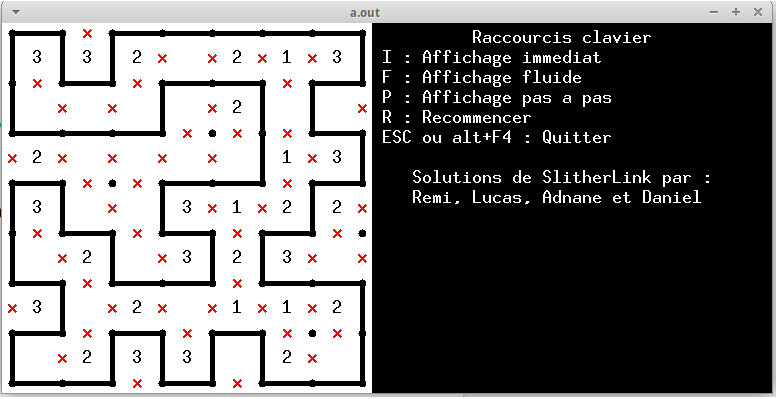
\includegraphics[scale=0.39]{slither.png}
\end{frame}

\section{Glade}

\begin{frame}{Glade}
    \begin{center}
    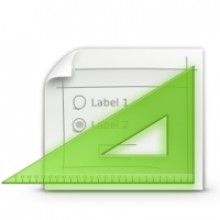
\includegraphics[scale=0.33]{glade_logo.png}
    \end{center}
    \begin{itemize}
    \item Glade est un outil de conception d'interfaces graphiques GTK+.
    \item on peut donc y développer visuellement son interface
    \item Glade génère un fichier XML
    \item on racorde notre interface à un fichier ".c":\\
    \hspace{0.3cm} \textbf{GtkBuilder *}builder;\\
    \hspace{0.3cm} builder=\textcolor{blue}{gtk\_builder\_new}();\\
    \hspace{0.3cm} \textcolor{blue}{gtk\_builder\_add\_from\_file}(builder, \textcolor{magenta}{"interface.xml"}, \&err);\\
    \end{itemize}
\end{frame}

\begin{frame}{Fin}
    \begin{center}
        Merci de votre attention!
    \end{center}
\end{frame}



\end{document}
